\chapter{Технологическая часть}

В данном разделе представлены средства реализации, структура программы и интерфейс ПО.

\section{Средства реализации}
Для разработки программы был выбран язык JavaScript --- мультипарадигменный язык программирования \cite{js}. Выбор данного языка обусловлен наличием опыта разработки с его использованием, наличием большого количество библиотек с открытым исходным кодом, направленных на визуализацию в трехмерном пространстве, а также большим количеством литературы по компьютерной графике ($\approx334000$ результатов по запросу <<js computer graphics algorithms>> в поисковой системе Google Академия).

Для создания пользовательского интерфейса программного обеспечения будет использоваться модуль datgui \cite{datgui}. Для мониторинга производительности будет использоваться модуль Stats \cite{stats}. Этот модуль позволяет отслеживать FPS (количество кадров в секунду). Данная информация поволит оценить производительность ПО. В качестве среды разработки выбран текстовый редактор Visual Studio Code \cite{vscode}, содержащий большое количеством плагинов и инструментов для различных языков программирования, в том числе для JavaScript. Такие инструменты облегчают и ускоряют процесс разработки программного обеспечения.

\section{Структура программы}
Разработанная программа состоит из следующих классов.
\begin{enumerate}[label=\arabic*)]
	\item  Сцена представляет собой объект класса $Scene$ с полями $camera$, $lights$, $cloth$
	\item  Ограничитель представляет собой объекта класса $Constraint$ с полями $p1$, $p2$ и $distance$.
	\item  Частица представляет объекта класса $Particle$ с полями $position$, $previous$, $original$.
	\item  Тканевая сетка представляет собой объект класса $Cloth$ с полями $particles$, $constraints$.
	\item  Источник света представляет собой объекта класса $DirectionalLight$ с полями $color$, $intensity$, $position$.
	\item  Камера представляет собой объекта класса $PerspectiveCamera$ с полями $position$, $lookAt$.
\end{enumerate}

%\begin{lstlisting}[label=raytracing1,caption=Реализация алгоритма испускания луча (начало), language=C++]
%Color MainWindow::_cast_ray(Color& buf_color, const Ray ray, const int depth)
%{
%	Intersection intersect;
	%
	%Color color;
%	
	%if (_scene.intersect(ray, intersect) && depth <= N) {
	%	QVector3D reflect_dir = _reflects(-ray.get_dst(), intersect.norm);
	%	reflect_dir.normalize();
	%	QVector3D reflect_orig = QVector3D::dotProduct(reflect_dir, intersect.norm) < 0 ? intersect.point - intersect.norm * EPS : intersect.point + intersect.norm * EPS;
	%	Color reflect_color;
	%	if (intersect.material.get_k_refl() > 0)
	%		reflect_color = _cast_ray(buf_color, Ray(reflect_orig, reflect_dir), depth + 1);
		
	%	QVector3D refract_dir = _refract(ray.get_dst(), intersect.norm, intersect.material.get_refraction_index());
	%	refract_dir.normalize();
	%	QVector3D refract_orig = QVector3D::dotProduct(refract_dir, intersect.norm) < 0 ? intersect.point - intersect.norm * EPS : intersect.point + intersect.norm * EPS;
	%	Color refract_color;
	%	if (intersect.material.get_k_refr() > 0)
	%		refract_color = _cast_ray(buf_color, Ray(refract_orig, refract_dir), depth + 1);
	%	color.r = (intersect.material.get_ambient().r * intersect.material.get_ka());
	%	color.g = (intersect.material.get_ambient().g * intersect.material.get_ka());
	%	color.b = (intersect.material.get_ambient().b * intersect.material.get_ka());
%\end{lstlisting}

\section{Интерфейс программного обеспечения}

На рисунках \ref{img:gui1} -- \ref{img:gui3} представлен интерфейс программы. При запуске загружается сцена с предварительно заданными объектами. Управление камерой производится с помощью компьютерной мыши путем зажатия левой кнопки мыши и передвижения в сторону. Для отдаления используется колесо мыши. Начальный интерфейс программного обеспечения отображен на рисунке \ref{img:gui1}.

\begin{table}[H]
	\centering
	\begin{tabular}{p{1\linewidth}}
		\centering
		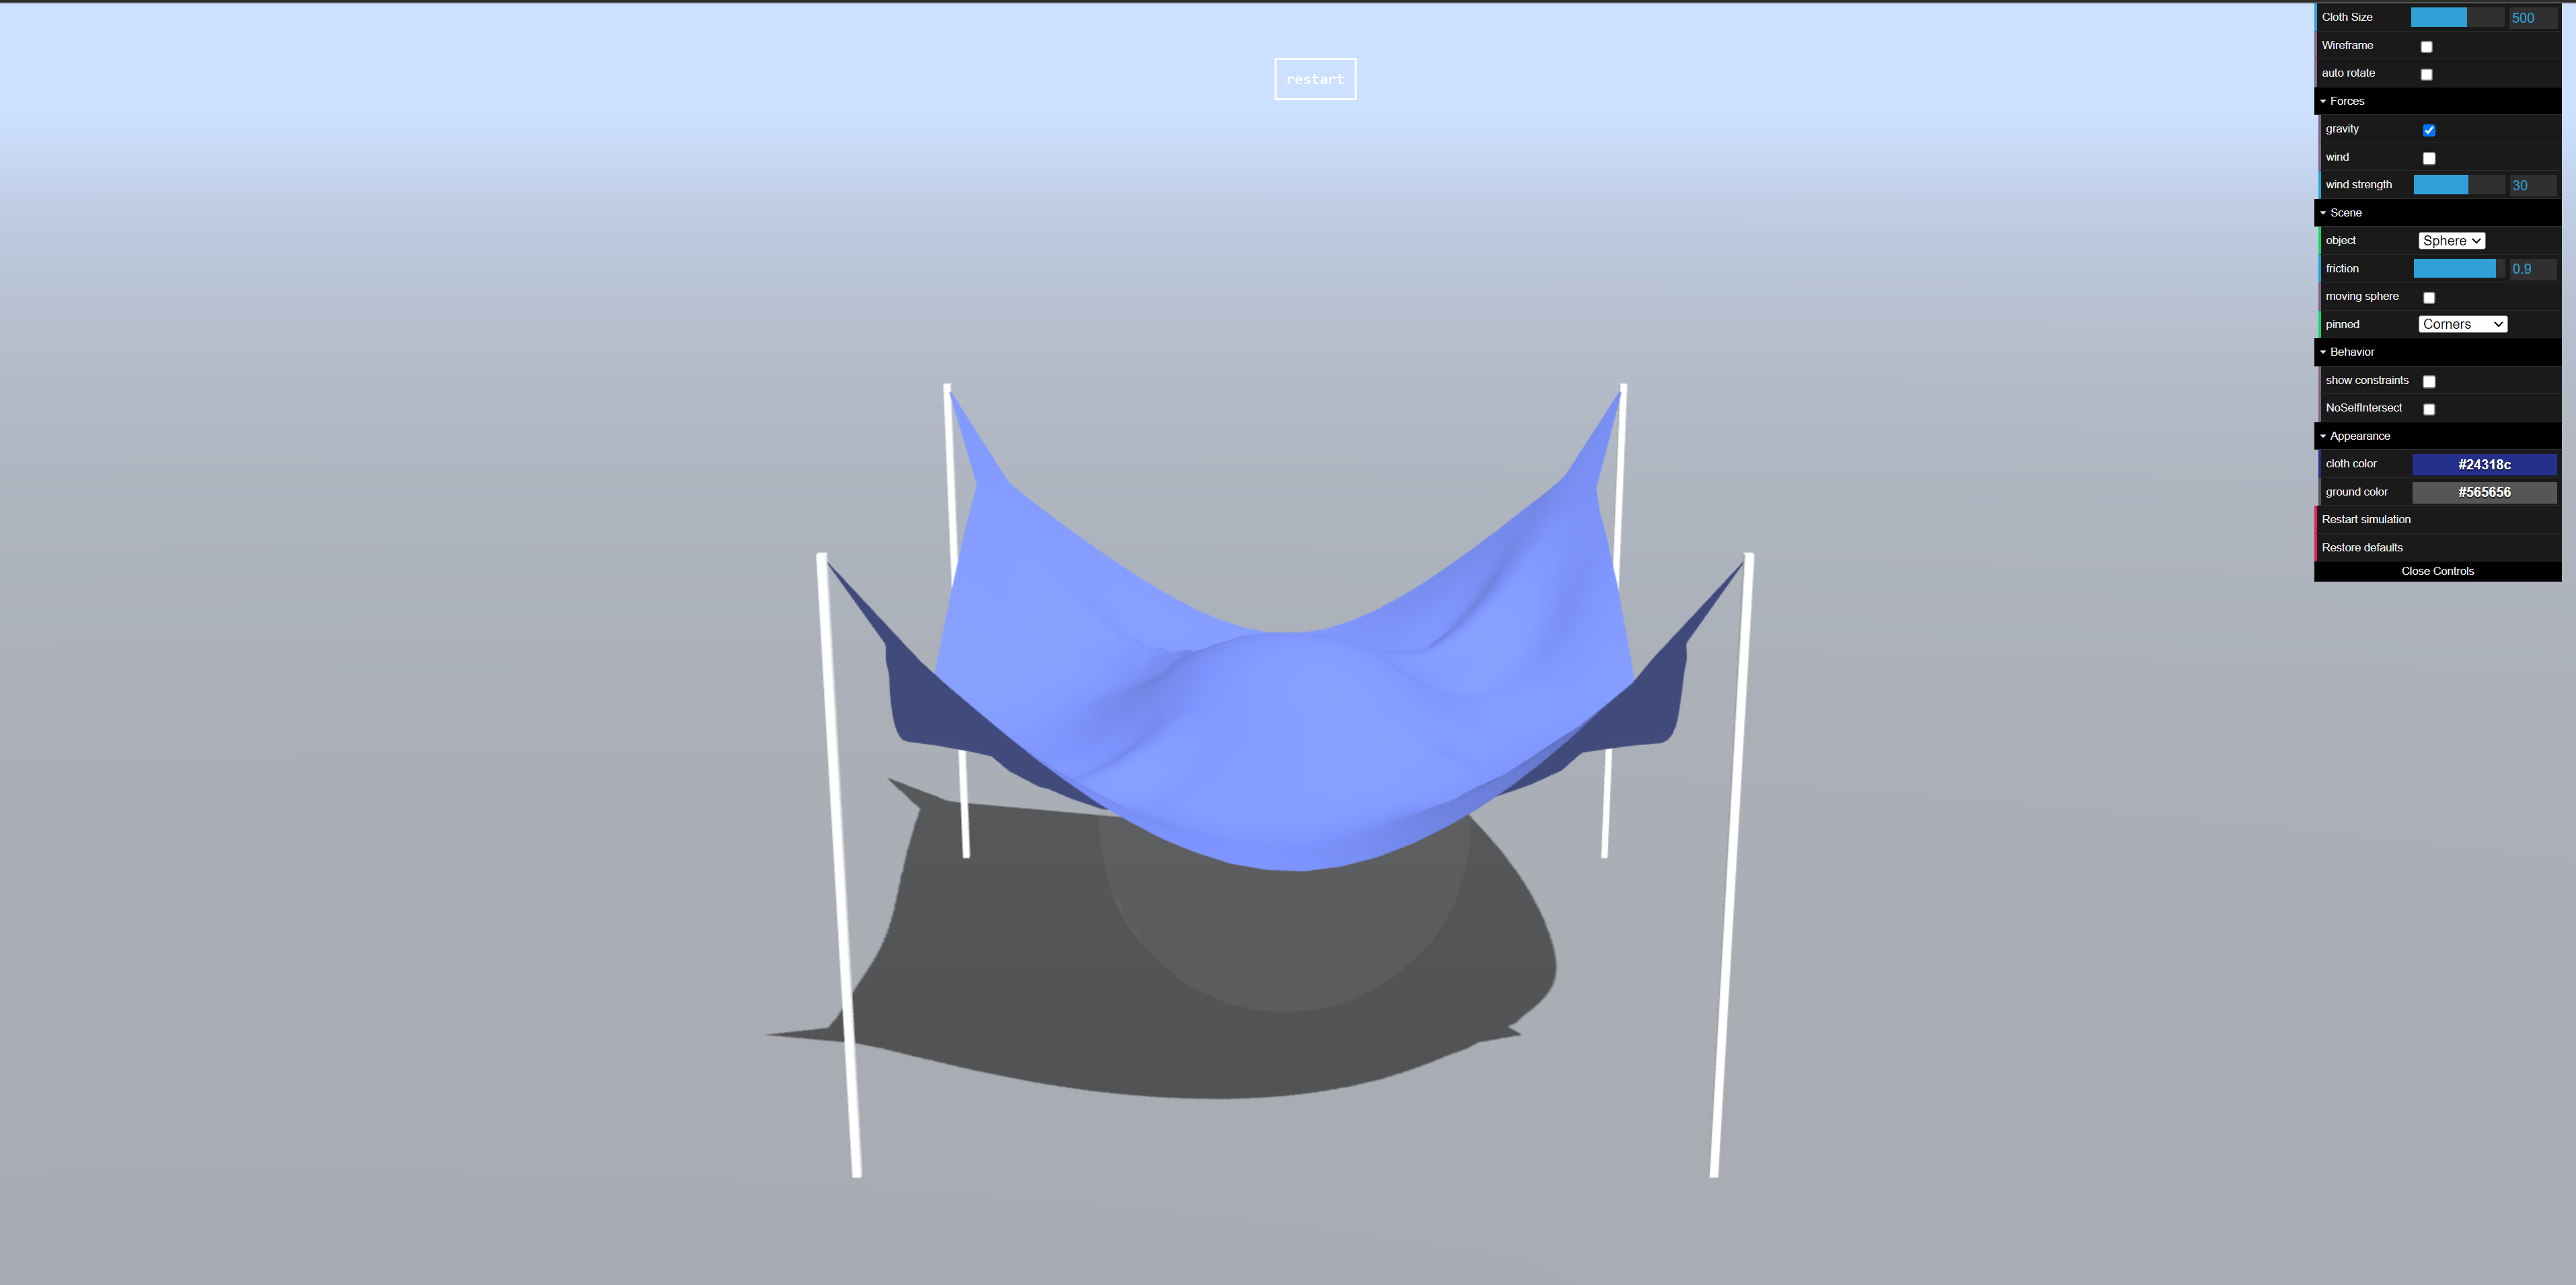
\includegraphics[width=0.95\linewidth]{include/gui1.png}
		\captionof{figure}{Интерфейс ПО (вид по умолчанию)}
		\label{img:gui1}
	\end{tabular}
\end{table}

В правом верхнем углу находится меню с настройками ткани и внешних сил. Для скрытия меню используется латинская буква <<H>>.Выпадающее меню представлено на рисунке \ref{img:gui2}.

\begin{table}[H]
	\centering
	\begin{tabular}{p{1\linewidth}}
		\centering
		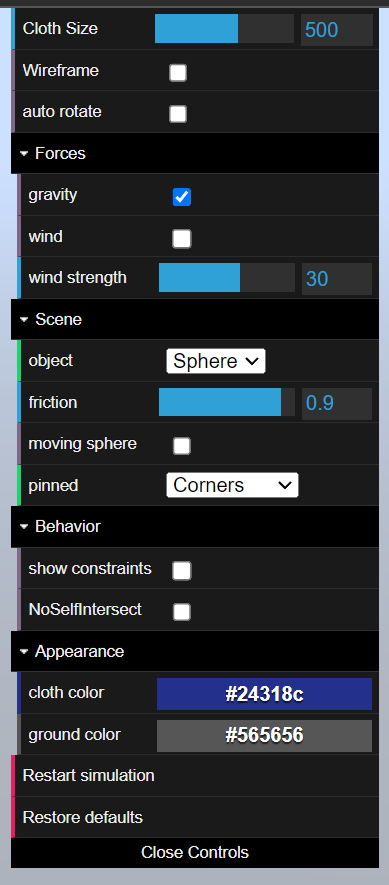
\includegraphics[height=0.65\linewidth]{include/gui2.png}
		\captionof{figure}{Интерфейс ПО (выпадающее меню)}
		\label{img:gui2}
	\end{tabular}
\end{table}
\clearpage
Пример измененных настроек представлен на рисунке \ref{img:gui3}.

\begin{table}[H]
	\centering
	\begin{tabular}{p{1\linewidth}}
		\centering
		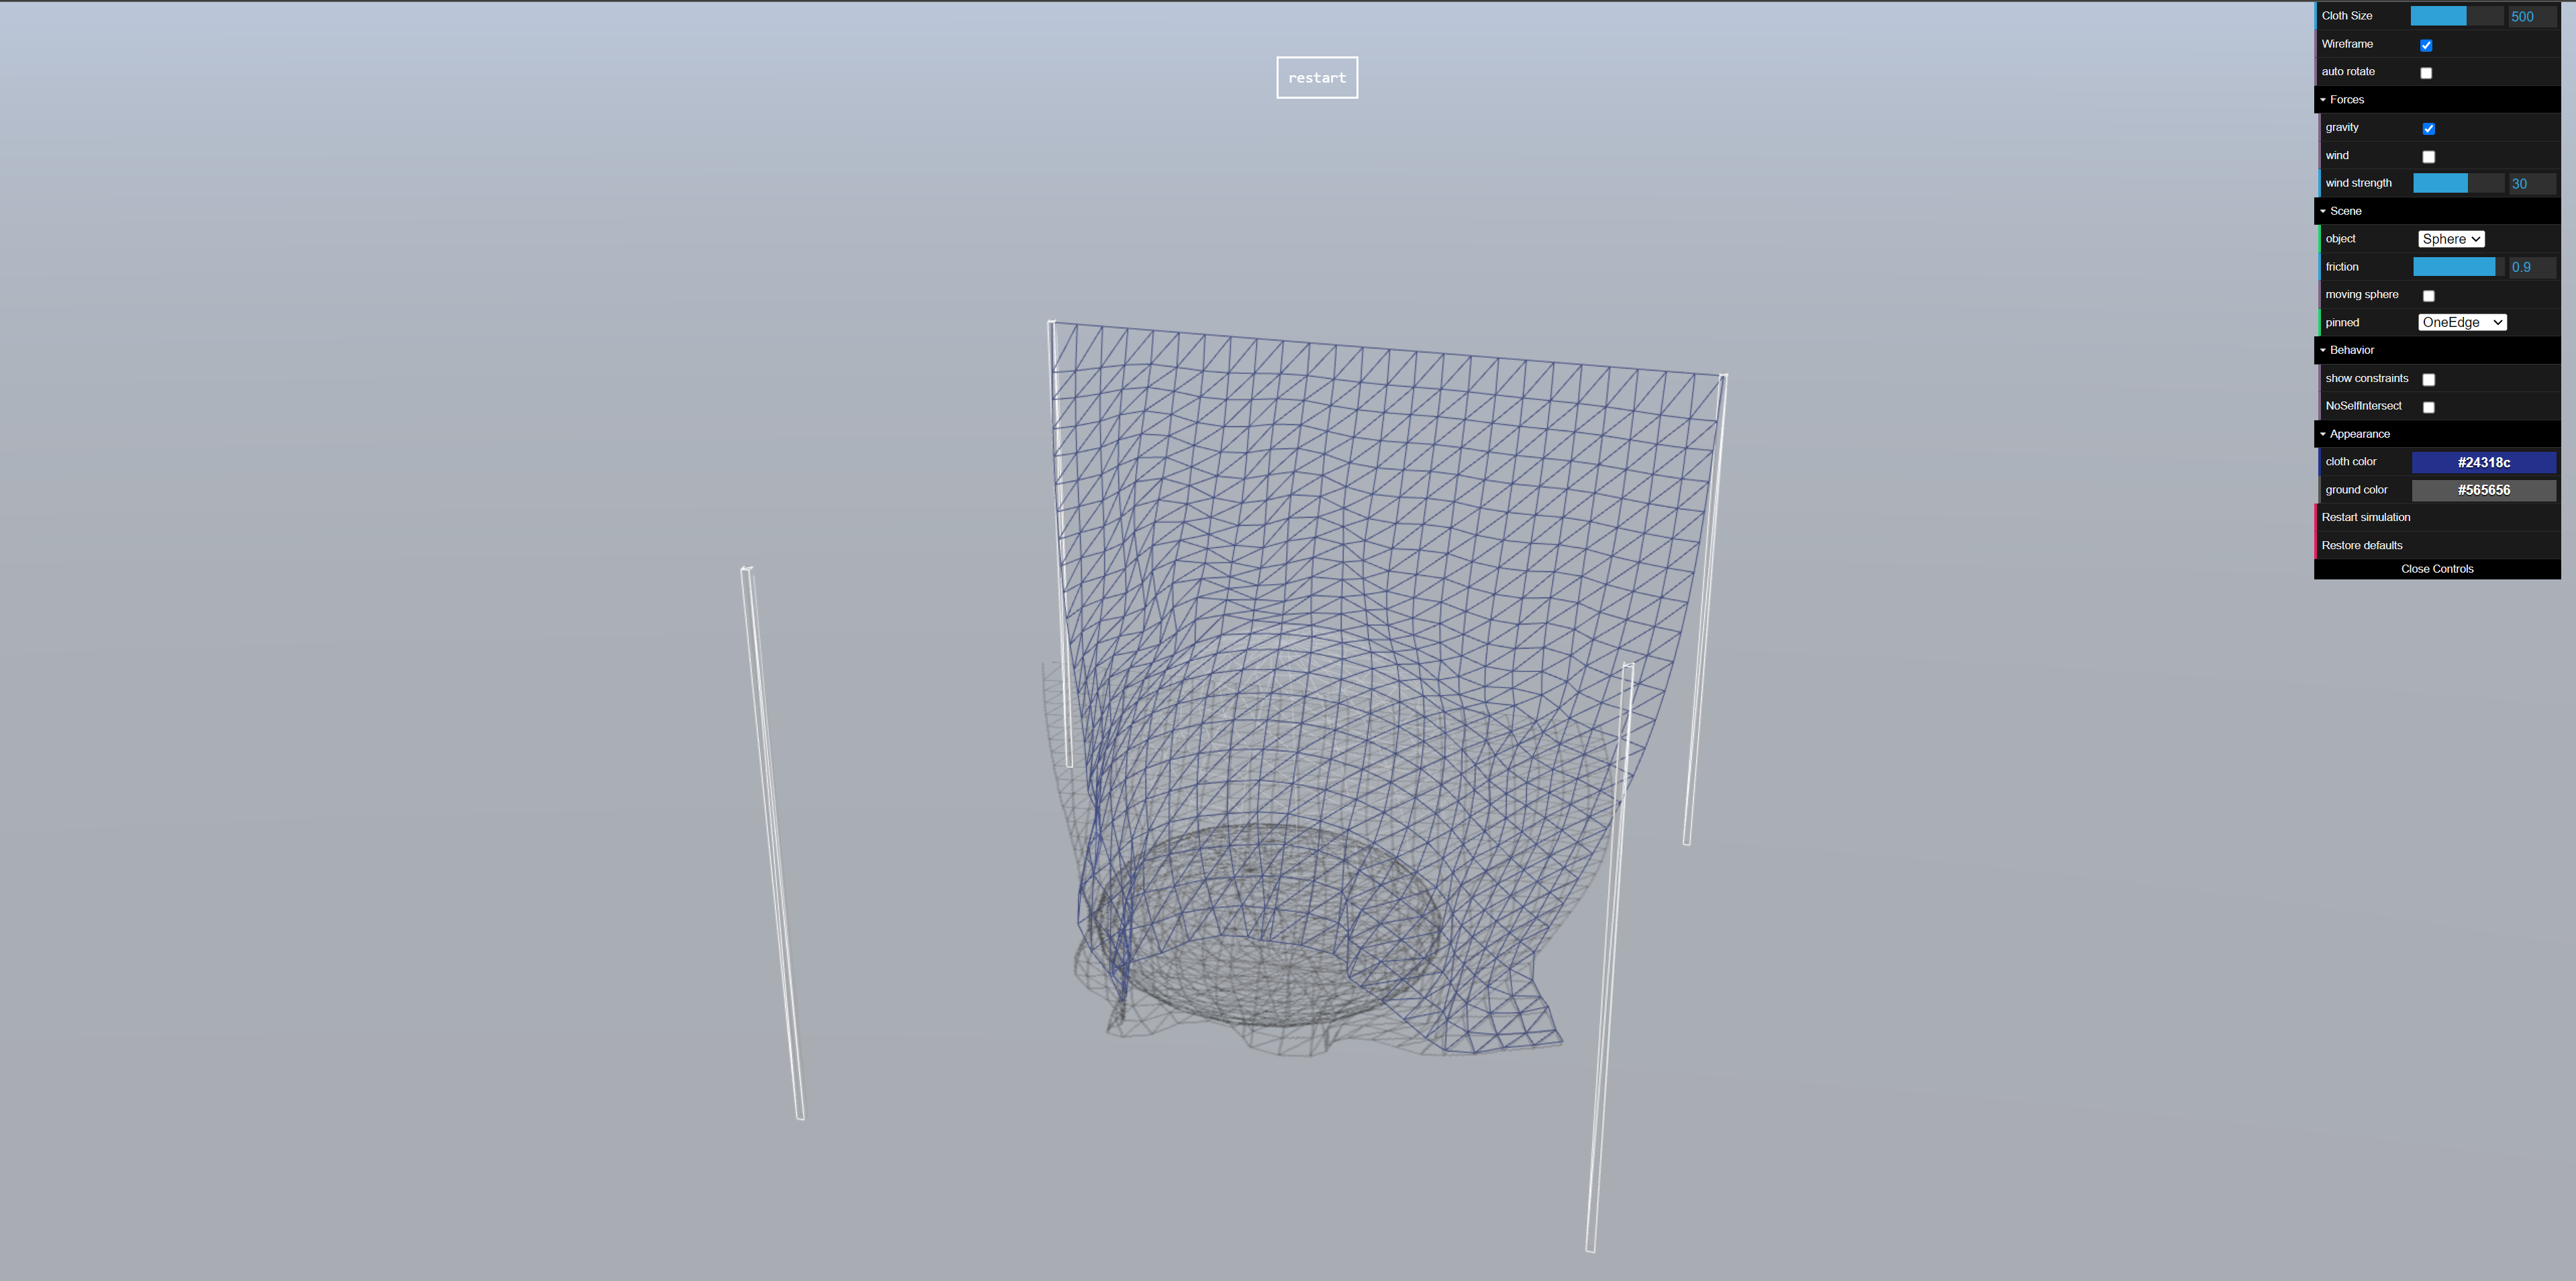
\includegraphics[width=0.95\linewidth]{include/gui3.png}
		\captionof{figure}{Интерфейс ПО (пример работы программы)}
		\label{img:gui3}
	\end{tabular}
\end{table}

\section*{Вывод}
\addcontentsline{toc}{section}{Вывод}
В данном разделе были выбраны и обоснованы средства реализации, описана структура программы, а также рассмотрен интерфейс программного обеспечения.
